\section{Background}


\subsection{DVMS}

\subsubsection{Overview}
DVMS~\cite{quesnel:cpe12}
(\emph{Distributed Virtual Machine Scheduler}) is a framework that enables VMs
to be scheduled cooperatively and dynamically in large scale distributed
systems.

DVMS is deployed as a set of agents that are organized following a ring
topology and that cooperate with one another to guarantee the quality of
service~(QoS) for the VMs.

When a node cannot guarantee the QoS for its hosted VMs or when it is
under-utilized, it starts an iterative scheduling procedure~(ISP) by querying
its neighbor to find a better placement; it thus becomes the initiator of the ISP.
If the request cannot be satisfied by the neighbor, it is forwarded to the
following free one until the ISP succeeds.
This approach allows each ISP to send requests only to a minimal
number of nodes, thus decreasing the scheduling time without requiring a
central point.
In addition, this approach allows several ISPs to occur independently at the
same moment throughout the infrastructure; in other words, scheduling is
performed on partitions of the system that are created dynamically, which
significantly improves the reactivity of the system.
Communications are handled efficiently, as each node involved in a partition
can forward a request directly to the first node outside its partition, by
means of a ``first out'' relation.

An example involving three partitions is shown on Figure~\ref{fig:isp}; in
particular, we can see the growth of partition~1 between two steps.
\begin{figure}[h!]
  \centering
  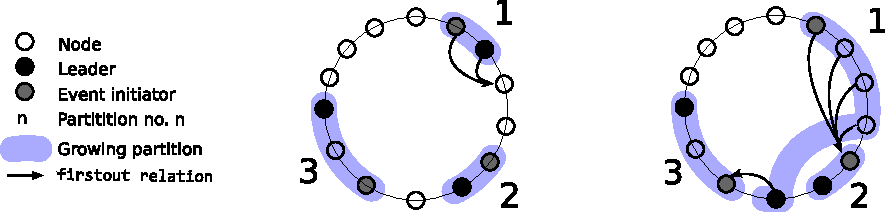
\includegraphics[width=0.9\linewidth]{Figures/resourceAcquisition-standard.pdf}
  \caption{Solving three problems simultaneously and independently with DVMS}%
  \label{fig:isp}%
\end{figure}

\subsubsection{Limitations}






\subsection{P2P - locality}

\begin{itemize}
	
	\item Vivaldi

	\item active/lazy clustering

\end{itemize}
